%
% ORIXES DA M�SICA: ORGANOLOX�A
% -----------------------------
\subsection{Organolox�a} \label{sub:organoloxia}

\begin{concepto}[\textit{Organolox�a: definici�n e caracter�sticas}]

A organolox�a � unha rama da Musicolox�a, que se ocupa do estudo e clasificaci�n dos instrumentos musicais con tres campos ben diferenciados:
	\begin{enumerate}[1)]
	\item
	\textbf{Investigaci�n} da orixe dos instrumentos, apoi�ndose na etnolox�a e antropolox�a, partindo principalmente de fontes iconogr�ficas.
	\item
	\textbf{Estudo pr�ctico} dos instrumentos en relaci�n �s s�as caracter�sticas e particularidades constructivas tendo en conta os materiais constructivos e diferentes t�cnicas interpretativas.
	\item
	\textbf{Clasificaci�n dos instrumentos} a partir dos puntos anteriores.  
	\end{enumerate} 

\end{concepto}

O sistema de clasificaci�n do belga \textbf{Mahillon} (1841-1924) inspirouno unha antiga colecci�n da India, con catro clases baseadas na natureza do material que vibra. 

A base para a investigaci�n organol�xica dos instrumentos musicais, est� baseada na clasificaci�n de Hornbostel-Sachs,\sidenote{No 1914, Erich von Hornbostel (1877-1935) e Curt Sachs (1881-1959) ampliaron o sistema, dando lugar ao que se utiliza hoxe en d�a con maior frecuencia.} que divide os instrumentos en catro familias xerais segundo a forma en que emiten as vibraci�ns que producen o son, distinguindo � vez cada unha delas en subgrupos\footnote{Hornbostel e Sachs, 1961} segundo a morfolox�a do instrumento. Esta clasificaci�n organol�xica\footnote{O {\scriptsize MIMO} (\emph{Musical Instrument Museums Online}) � a entidade encargada de revisi�n e recentemente engadeu novos subgrupos.} � a m�is empregada, malia que non faltan cr�ticas a este sistema.




%\begin{figure}[h!]
%\centering
%\subfigure[Frauta primitiva]{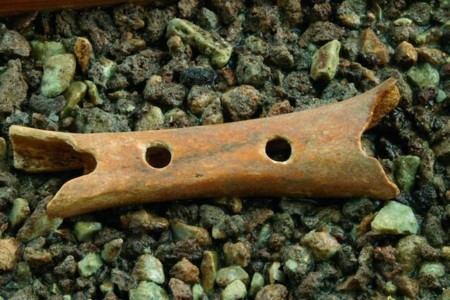
\includegraphics[scale=0.5]{../figures/ud-00/frauta-oso.jpg}}
%\subfigure[Tambor primitivo]{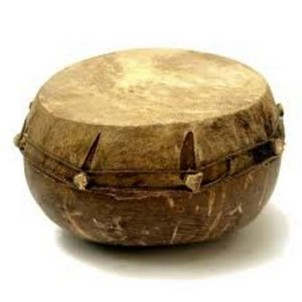
\includegraphics[scale=0.5]{../figures/ud-00/tambor-primitivo.jpeg}}
%\subfigure[Bramadera primitiva]{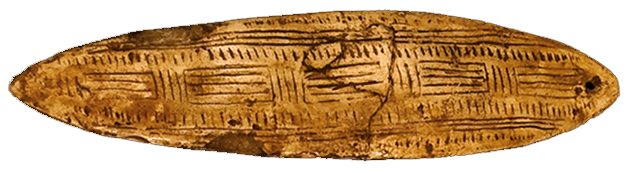
\includegraphics[scale=0.5]{../figures/ud-00/bramadera-primitiva.png}}
%\subfigure[Frauta de �so]{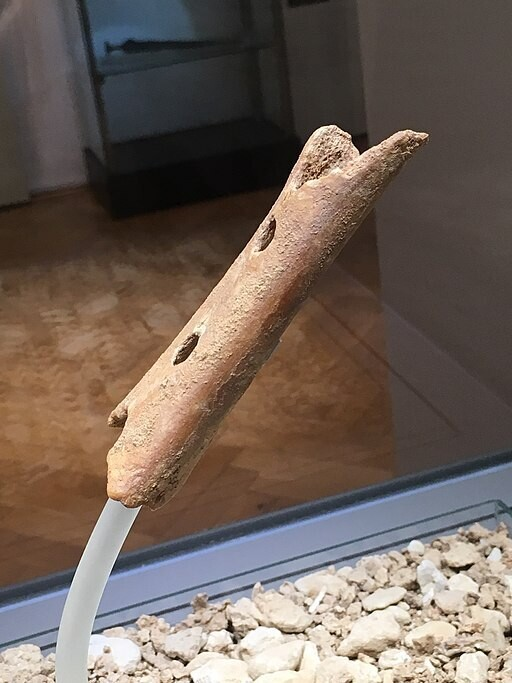
\includegraphics[scale=0.25]{../figures/ud-00/frauta-oso-museo.jpg}}
%\caption{Instrumentos primitivos}
%\label{fig:instrumentos-prehistoricos}
%\end{figure}


